% Archivo de caracterización de infraestructura corregido

% Torre HP 1
\begin{table}[H]
\centering
\caption{Ficha técnica --- Torre 1}\label{tab:torre-hp-1}
\begin{tabular}{|p{0.6\textwidth}|p{0.3\textwidth}|}
\hline
\multicolumn{2}{|l|}{\textbf{DESCRIPCIÓN FÍSICA:} Servidor tipo torre} \\ \hline
\textbf{TIPO DE RECURSO:} Torre &
\multirow{5}{*}{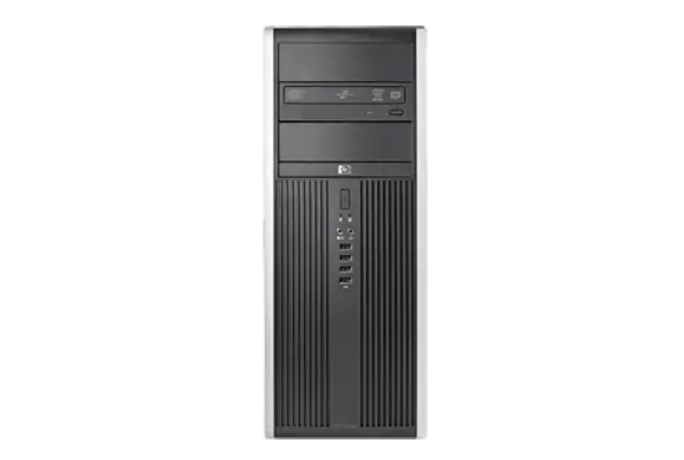
\includegraphics[width=0.25\textwidth,height=4cm,keepaspectratio]{tablas-images/cp1/torres/torre-1.png}} \\ \cline{1-1}
\textbf{MODELO:} Desconocido & \\ \cline{1-1}
\textbf{MARCA:} HP & \\ \cline{1-1}
\textbf{CÓDIGO DE INVENTARIO:} 7 24390 49867 3 & \\ \cline{1-1}
\textbf{NÚMERO EN CPD:} 14 & \\ \hline
\multicolumn{2}{|l|}{\textbf{ESPECIFICACIONES TÉCNICAS}} \\ \hline
\multicolumn{2}{|p{0.95\textwidth}|}{
\footnotesize
- 8 entradas USB (4 al frente, 4 en la parte trasera)
- Entrada de audio y microfono
- Entrada HDMI
- Lector de DVDs
- 3 puertos Ethernet (Parte trasera)
- Entrada Displayport
- Puertos PS/2 (Teclado y Ratón)
} \\ \hline
\multicolumn{2}{|l|}{\textbf{PROPÓSITO:} Hipervisor de XCP-ng} \\ \hline
\multicolumn{2}{|l|}{\textbf{OPORTUNIDAD DE USO:} Proyectos del \GRID} \\ \hline
\multicolumn{2}{|p{0.9\textwidth}|}{\textbf{OBSERVACIONES:} El Equipo no tiene modelo. El equipo está diseñado para usuario final pero fue adaptado para entornos de virtualización.} \\ \hline
\end{tabular}
\end{table}


% Torre 2
\begin{table}[H]
\centering
\caption{Ficha técnica --- Torre 2}\label{tab:torre-2}
\begin{tabular}{|p{0.6\textwidth}|p{0.3\textwidth}|}
\hline
\multicolumn{2}{|l|}{\textbf{DESCRIPCIÓN FÍSICA:} Servidor tipo torre} \\ \hline
\textbf{TIPO DE RECURSO:} Torre & 
\multirow{5}{*}{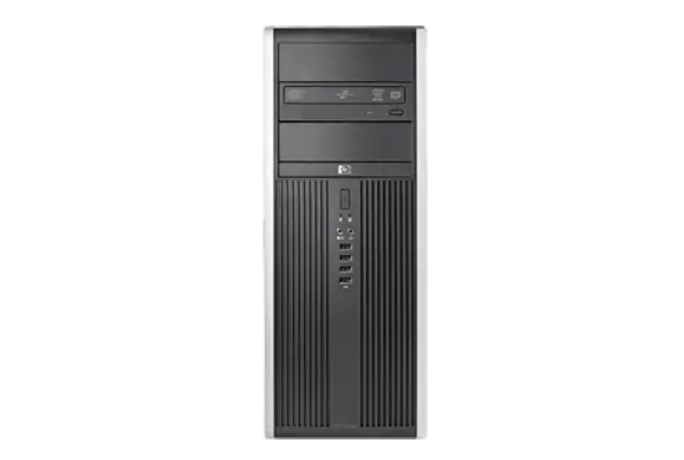
\includegraphics[width=0.25\textwidth,height=4cm,keepaspectratio]{tablas-images/cp1/torres/torre-1.png}} \\ \cline{1-1}
\textbf{MODELO:} Desconocido & \\ \cline{1-1}
\textbf{MARCA:} HP & \\ \cline{1-1}
\textbf{CÓDIGO DE INVENTARIO:} 7 24390 49861 1 & \\ \cline{1-1}
\textbf{NÚMERO EN CPD:} 12 & \\ \hline
\multicolumn{2}{|l|}{\textbf{ESPECIFICACIONES TÉCNICAS}} \\ \hline
\multicolumn{2}{|p{0.95\textwidth}|}{
\footnotesize
- 8 entradas USB (4 al frente, 4 en la parte trasera)
- Entrada de audio y microfono
- Entrada HDMI
- Lector de DVDs
- 3 puertos Ethernet (Parte trasera)
- Entrada Displayport
- Puertos PS/2 (Teclado y Ratón)
} \\ \hline
\multicolumn{2}{|l|}{\textbf{PROPÓSITO:} Hipervisor de XCP-ng} \\ \hline
\multicolumn{2}{|l|}{\textbf{OPORTUNIDAD DE USO:} Proyectos del \GRID} \\ \hline
\multicolumn{2}{|p{0.9\textwidth}|}{\textbf{OBSERVACIONES:} El Equipo no tiene modelo. El equipo está diseñado para usuario final pero fue adaptado para entornos de virtualización.} \\ \hline
\end{tabular}
\end{table}

% Torre 3
\begin{table}[H]
\centering
\caption{Ficha técnica -- Torre 3}
\label{tab:torre-3}
\begin{tabular}{|p{0.6\textwidth}|p{0.3\textwidth}|}
\hline
\multicolumn{2}{|l|}{\textbf{DESCRIPCIÓN FÍSICA:} Servidor tipo torre} \\ \hline
\textbf{TIPO DE RECURSO:} Torre & 
\multirow{5}{*}{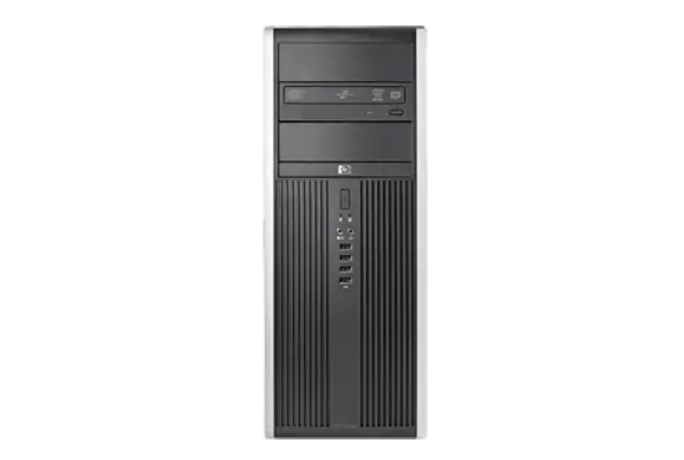
\includegraphics[width=0.25\textwidth,height=4cm,keepaspectratio]{tablas-images/cp1/torres/torre-1.png}} \\ \cline{1-1}
\textbf{MODELO:} Desconocido & \\ \cline{1-1}
\textbf{MARCA:} HP & \\ \cline{1-1}
\textbf{CÓDIGO DE INVENTARIO:} 7 24390 49969 4 & \\ \cline{1-1}
\textbf{NÚMERO EN CPD:} 13 & \\ \hline
\multicolumn{2}{|l|}{\textbf{ESPECIFICACIONES TÉCNICAS}} \\ \hline
\multicolumn{2}{|p{0.95\textwidth}|}{
\footnotesize
- 8 entradas USB (4 al frente, 4 en la parte trasera)
- Entrada de audio y microfono
- Entrada HDMI
- Lector de DVDs
- 3 puertos Ethernet (Parte trasera)
- Entrada Displayport
- Puertos PS/2 (Teclado y Ratón)
} \\ \hline
\multicolumn{2}{|l|}{\textbf{PROPÓSITO:} Hipervisor de XCP-ng} \\ \hline
\multicolumn{2}{|l|}{\textbf{OPORTUNIDAD DE USO:} Proyectos del \GRID} \\ \hline
\multicolumn{2}{|p{0.9\textwidth}|}{\textbf{OBSERVACIONES:} El Equipo no tiene modelo. El equipo está diseñado para usuario final pero fue adaptado para entornos de virtualización.} \\ \hline
\end{tabular}
\end{table}

% Torre 4
\begin{table}[H]
\centering
\caption{Ficha técnica --- Torre 4}\label{tab:torre-4}
\begin{tabular}{|p{0.6\textwidth}|p{0.3\textwidth}|}
\hline
\multicolumn{2}{|l|}{\textbf{DESCRIPCIÓN FÍSICA:} Servidor tipo torre} \\ \hline
\textbf{TIPO DE RECURSO:} Torre & 
\multirow{5}{*}{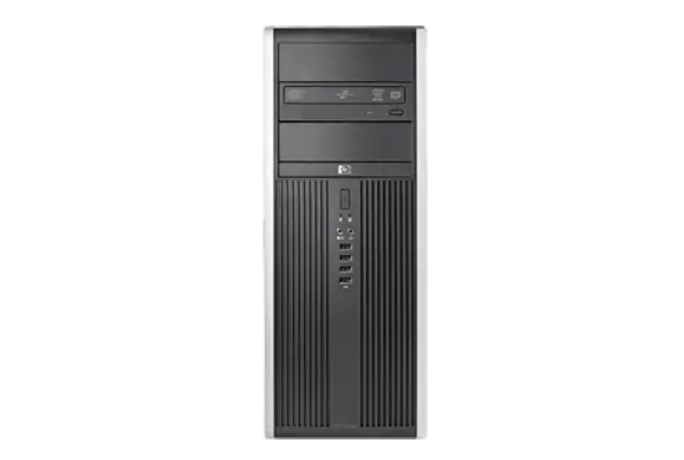
\includegraphics[width=0.25\textwidth,height=4cm,keepaspectratio]{tablas-images/cp1/torres/torre-1.png}} \\ \cline{1-1}
\textbf{MODELO:} Desconocido & \\ \cline{1-1}
\textbf{MARCA:} HP & \\ \cline{1-1}
\textbf{CÓDIGO DE INVENTARIO:} 7 24390 49879 4 & \\ \cline{1-1}
\textbf{NÚMERO EN CPD:} 14 & \\ \hline
\multicolumn{2}{|l|}{\textbf{ESPECIFICACIONES TÉCNICAS}} \\ \hline
\multicolumn{2}{|p{0.95\textwidth}|}{
\footnotesize
- 8 entradas USB (4 al frente, 4 en la parte trasera)
- Entrada de audio y microfono
- Entrada HDMI
- Lector de DVDs
- 3 puertos Ethernet (Parte trasera)
- Entrada Displayport
- Puertos PS/2 (Teclado y Ratón)
} \\ \hline
\multicolumn{2}{|l|}{\textbf{PROPÓSITO:} Hipervisor de XCP-ng} \\ \hline
\multicolumn{2}{|l|}{\textbf{OPORTUNIDAD DE USO:} Proyectos del \GRID} \\ \hline
\multicolumn{2}{|p{0.9\textwidth}|}{\textbf{OBSERVACIONES:} El Equipo no tiene modelo. El equipo está diseñado para usuario final pero fue adaptado para entornos de virtualización.} \\ \hline
\end{tabular}
\end{table}

% Torre 5
\begin{table}[H]
\centering
\caption{Ficha técnica --- Torre 5}
\label{tab:torre-5}
\begin{tabular}{|p{0.6\textwidth}|p{0.3\textwidth}|}
\hline
\multicolumn{2}{|l|}{\textbf{DESCRIPCIÓN FÍSICA:} Servidor tipo torre} \\ \hline
\textbf{TIPO DE RECURSO:} Torre & 
\multirow{5}{*}{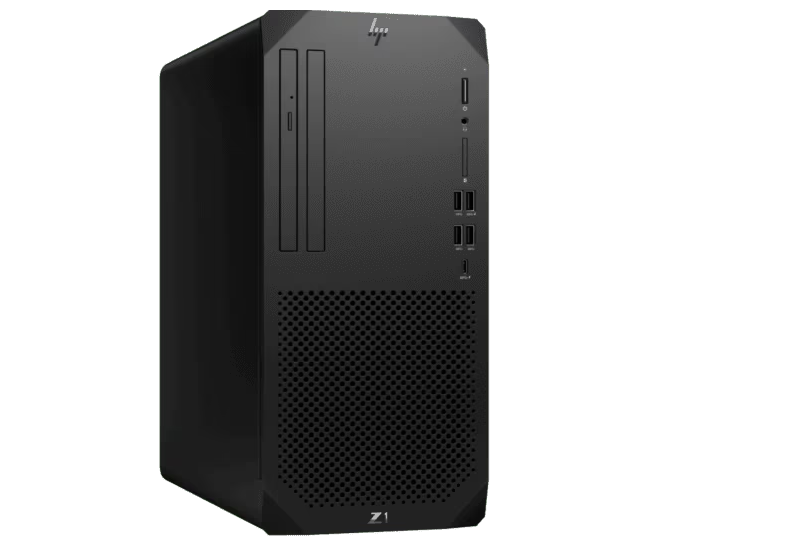
\includegraphics[width=0.25\textwidth,height=4cm,keepaspectratio]{tablas-images/cp1/torres/torre-2.png}} \\ \cline{1-1}
\textbf{MODELO:} G9 & \\ \cline{1-1}
\textbf{MARCA:} HP & \\ \cline{1-1}
\textbf{CÓDIGO DE INVENTARIO:} 72992 & \\ \cline{1-1}
\textbf{NÚMERO EN CPD:} 22 & \\ \hline
\multicolumn{2}{|l|}{\textbf{ESPECIFICACIONES TÉCNICAS}} \\ \hline
\multicolumn{2}{|p{0.95\textwidth}|}{
\footnotesize
- 9 entradas USB (4 al frente, 5 en la parte trasera)
- Entrada de audio y microfono
- Entrada HDMI
- Lector de DVDs
- 1 puerto Ethernet (Parte trasera)
- 2 Entrada Displayport
- Procesador Intel vPro i9
} \\ \hline
\multicolumn{2}{|l|}{\textbf{PROPÓSITO:} Hipervisor de XCP-ng} \\ \hline
\multicolumn{2}{|l|}{\textbf{OPORTUNIDAD DE USO:} Proyectos del \GRID} \\ \hline
\multicolumn{2}{|p{0.9\textwidth}|}{\textbf{OBSERVACIONES:} El equipo está diseñado para usuario final pero fue adaptado para entornos de virtualización.} \\ \hline
\end{tabular}
\end{table}

% Torre 6
\begin{table}[H]
\centering
\caption{Ficha técnica --- Torre 6}
\label{tab:torre-6}
\begin{tabular}{|p{0.6\textwidth}|p{0.3\textwidth}|}
\hline
\multicolumn{2}{|l|}{\textbf{DESCRIPCIÓN FÍSICA:} Servidor tipo torre} \\ \hline
\textbf{TIPO DE RECURSO:} Torre & 
\multirow{5}{*}{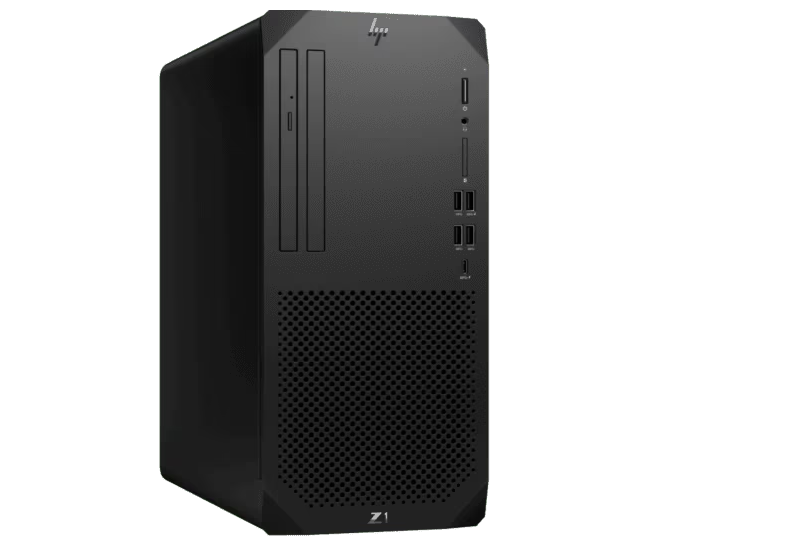
\includegraphics[width=0.25\textwidth,height=4cm,keepaspectratio]{tablas-images/cp1/torres/torre-2.png}} \\ \cline{1-1}
\textbf{MODELO:} G9 & \\ \cline{1-1}
\textbf{MARCA:} HP & \\ \cline{1-1}
\textbf{CÓDIGO DE INVENTARIO:} 72976 & \\ \cline{1-1}
\textbf{NÚMERO EN CPD:} 21 & \\ \hline
\multicolumn{2}{|l|}{\textbf{ESPECIFICACIONES TÉCNICAS}} \\ \hline
\multicolumn{2}{|p{0.95\textwidth}|}{
\footnotesize
- 9 entradas USB (4 al frente, 5 en la parte trasera)
- Entrada de audio y microfono
- Entrada HDMI
- Lector de DVDs
- 1 puerto Ethernet (Parte trasera)
- 2 Entrada Displayport
- Procesador Intel vPro i9
} \\ \hline
\multicolumn{2}{|l|}{\textbf{PROPÓSITO:} Hipervisor de XCP-ng} \\ \hline
\multicolumn{2}{|l|}{\textbf{OPORTUNIDAD DE USO:} Proyectos del \GRID} \\ \hline
\multicolumn{2}{|p{0.9\textwidth}|}{\textbf{OBSERVACIONES:} El equipo está diseñado para usuario final pero fue adaptado para entornos de virtualización.} \\ \hline
\end{tabular}
\end{table}


% Torre 7
\begin{table}[H]
\centering
\caption{Ficha técnica --- Torre 7}
\label{tab:torre-7}
\begin{tabular}{|p{0.6\textwidth}|p{0.3\textwidth}|}
\hline
\multicolumn{2}{|l|}{\textbf{DESCRIPCIÓN FÍSICA:} Servidor tipo torre} \\ \hline
\textbf{TIPO DE RECURSO:} Torre & 
\multirow{5}{*}{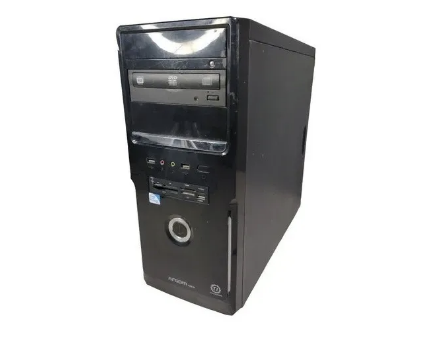
\includegraphics[width=0.25\textwidth,height=4cm,keepaspectratio]{tablas-images/cp1/torres/ATX.png}} \\ \cline{1-1}
\textbf{MODELO:} Argom tech & \\ \cline{1-1}
\textbf{MARCA:} Argom tech & \\ \cline{1-1}
\textbf{CÓDIGO DE INVENTARIO:} Sin código & \\ \cline{1-1}
\textbf{NÚMERO EN CPD:} 11 & \\ \hline
\multicolumn{2}{|l|}{\textbf{ESPECIFICACIONES TÉCNICAS}} \\ \hline
\multicolumn{2}{|p{0.95\textwidth}|}{
\footnotesize
-Procesador: INTEL PENTIUM 62030 3.00GHz
-Arquitectura: X64
-Ram: 16GB
-Disco: 1024GB
-Unidad de CDI/DVD: SI
-Tarjeta de video: Integrada
-Tarjeta de sonido: Integrada
} \\ \hline
\multicolumn{2}{|l|}{\textbf{PROPÓSITO:} Hipervisor de XCP-ng} \\ \hline
\multicolumn{2}{|l|}{\textbf{OPORTUNIDAD DE USO:} Proyectos del \GRID} \\ \hline
\multicolumn{2}{|p{0.9\textwidth}|}{\textbf{OBSERVACIONES:} El equipo está diseñado para usuario final pero fue adaptado para entornos de virtualización.} \\ \hline
\end{tabular}
\end{table}



% Rack 1
\begin{table}[H]
\centering
\caption{Ficha técnica --- Rack 1}
\label{tab:rack-1}
\begin{tabular}{|p{0.6\textwidth}|p{0.3\textwidth}|}
\hline
\multicolumn{2}{|l|}{\textbf{DESCRIPCIÓN FÍSICA:} Servidor tipo rack} \\ \hline
\textbf{TIPO DE RECURSO:} Servidor & 
\multirow{5}{*}{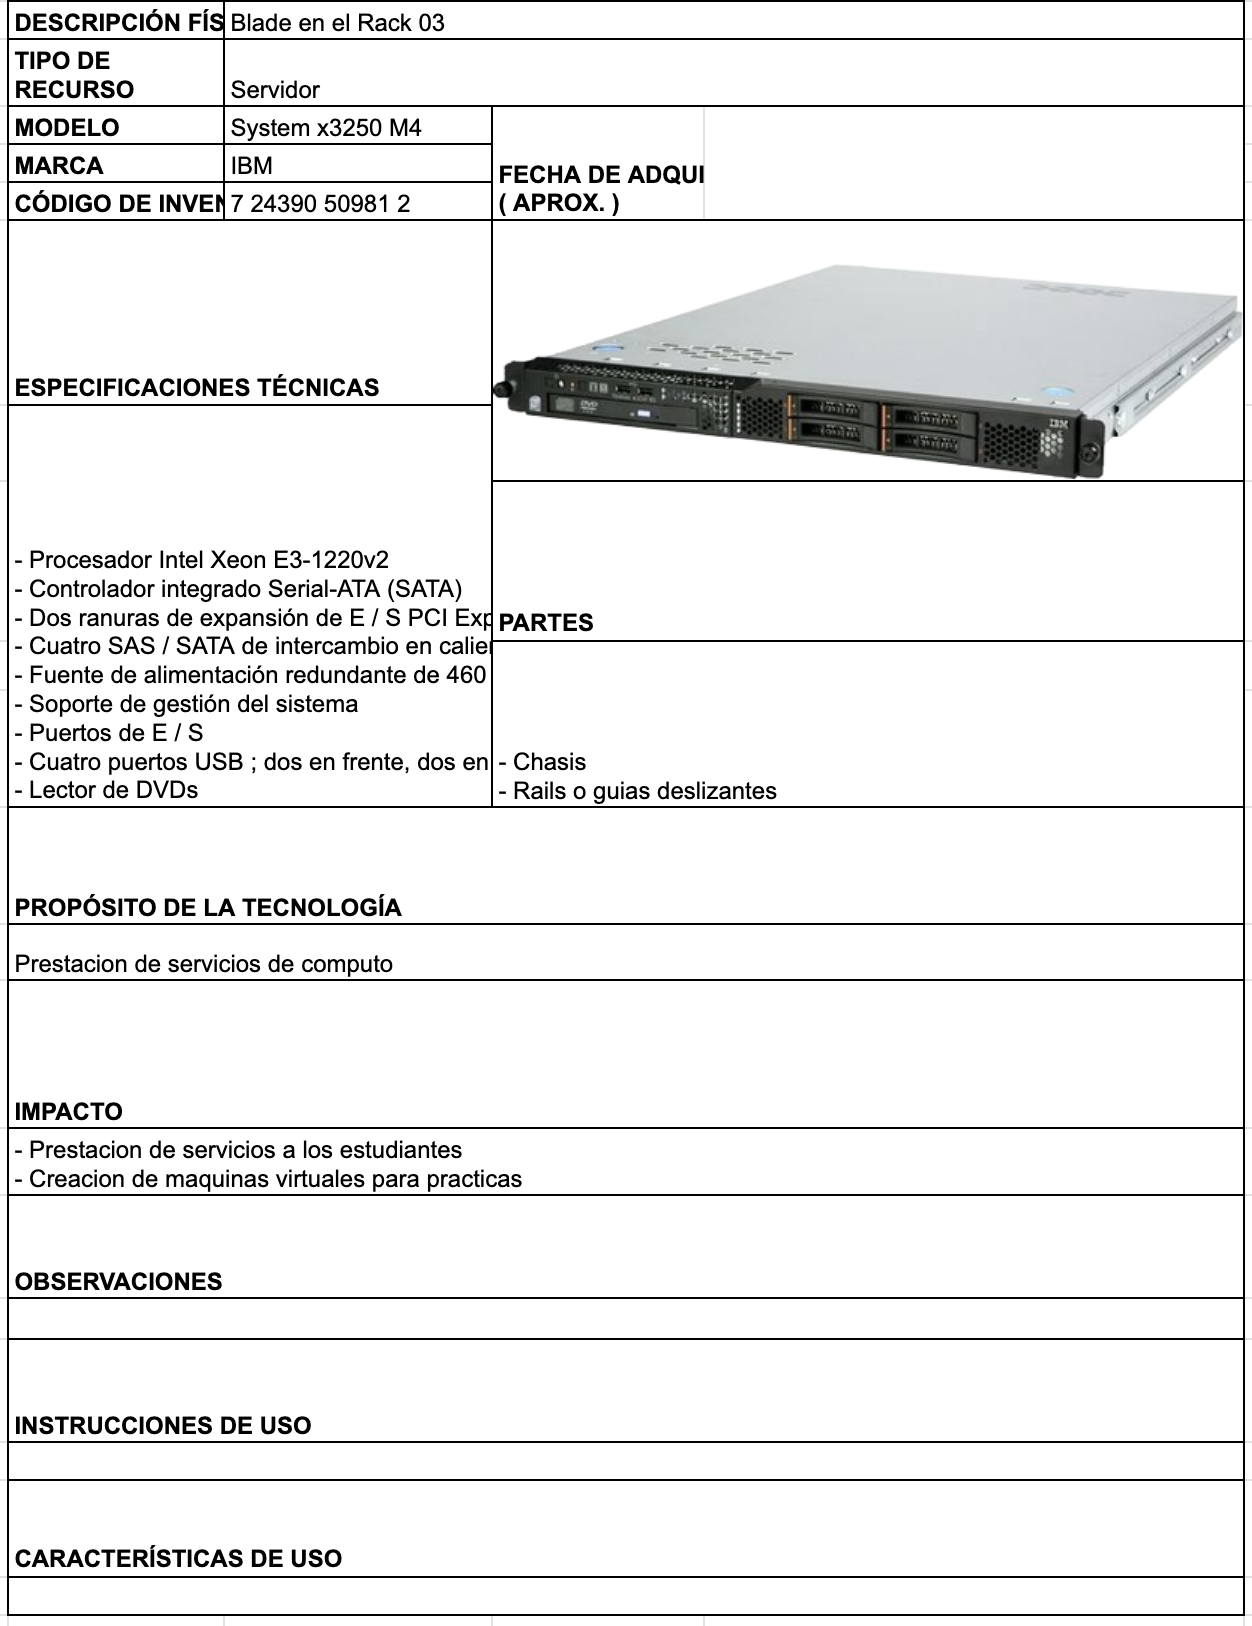
\includegraphics[width=0.25\textwidth,height=4cm,keepaspectratio]{tablas-images/cp1/racks/rack-1.png}} \\ \cline{1-1}
\textbf{MODELO:} System x3250 M4 & \\ \cline{1-1}
\textbf{MARCA:} IBM & \\ \cline{1-1}
\textbf{CÓDIGO DE INVENTARIO:} 7 24390 50981  & \\ \cline{1-1}
\textbf{NUMERO EN CPD:} 55 & \\ \hline
\multicolumn{2}{|l|}{\textbf{ESPECIFICACIONES TÉCNICAS}} \\ \hline
\multicolumn{2}{|p{0.95\textwidth}|}{
\footnotesize
- Procesador Intel Xeon E3-1220v2
- Controlador integrado Serial-ATA (SATA)
- Dos ranuras de expansión de E / S PCI Express
- Cuatro SAS / SATA de intercambio en caliente de 2,5 pulgadas
- Fuente de alimentación redundante de 460 vatios
- Soporte de gestión del sistema
- Puertos de E / S
- Cuatro puertos USB ; dos en frente, dos en la parte trasera
- Lector de DVDs
} \\ \hline
\multicolumn{2}{|l|}{\textbf{PROPÓSITO:} Prestacion de servicios de computo} \\ \hline
\multicolumn{2}{|p{0.9\textwidth}|}{\textbf{IMPACTO:} - Prestacion de servicios a los estudiantes
- Creacion de maquinas virtuales para practicas} \\ \hline
\multicolumn{2}{|p{0.9\textwidth}|}{\textbf{OBSERVACIONES:} Ninguna} \\ \hline
\end{tabular}
\end{table}

% Rack 2
\begin{table}[H]
\centering
\caption{Ficha técnica --- Rack 2}
\label{tab:rack-2}
\begin{tabular}{|p{0.6\textwidth}|p{0.3\textwidth}|}
\hline
\multicolumn{2}{|l|}{\textbf{DESCRIPCIÓN FÍSICA:} Servidor tipo rack} \\ \hline
\textbf{TIPO DE RECURSO:} Servidor & 
\multirow{5}{*}{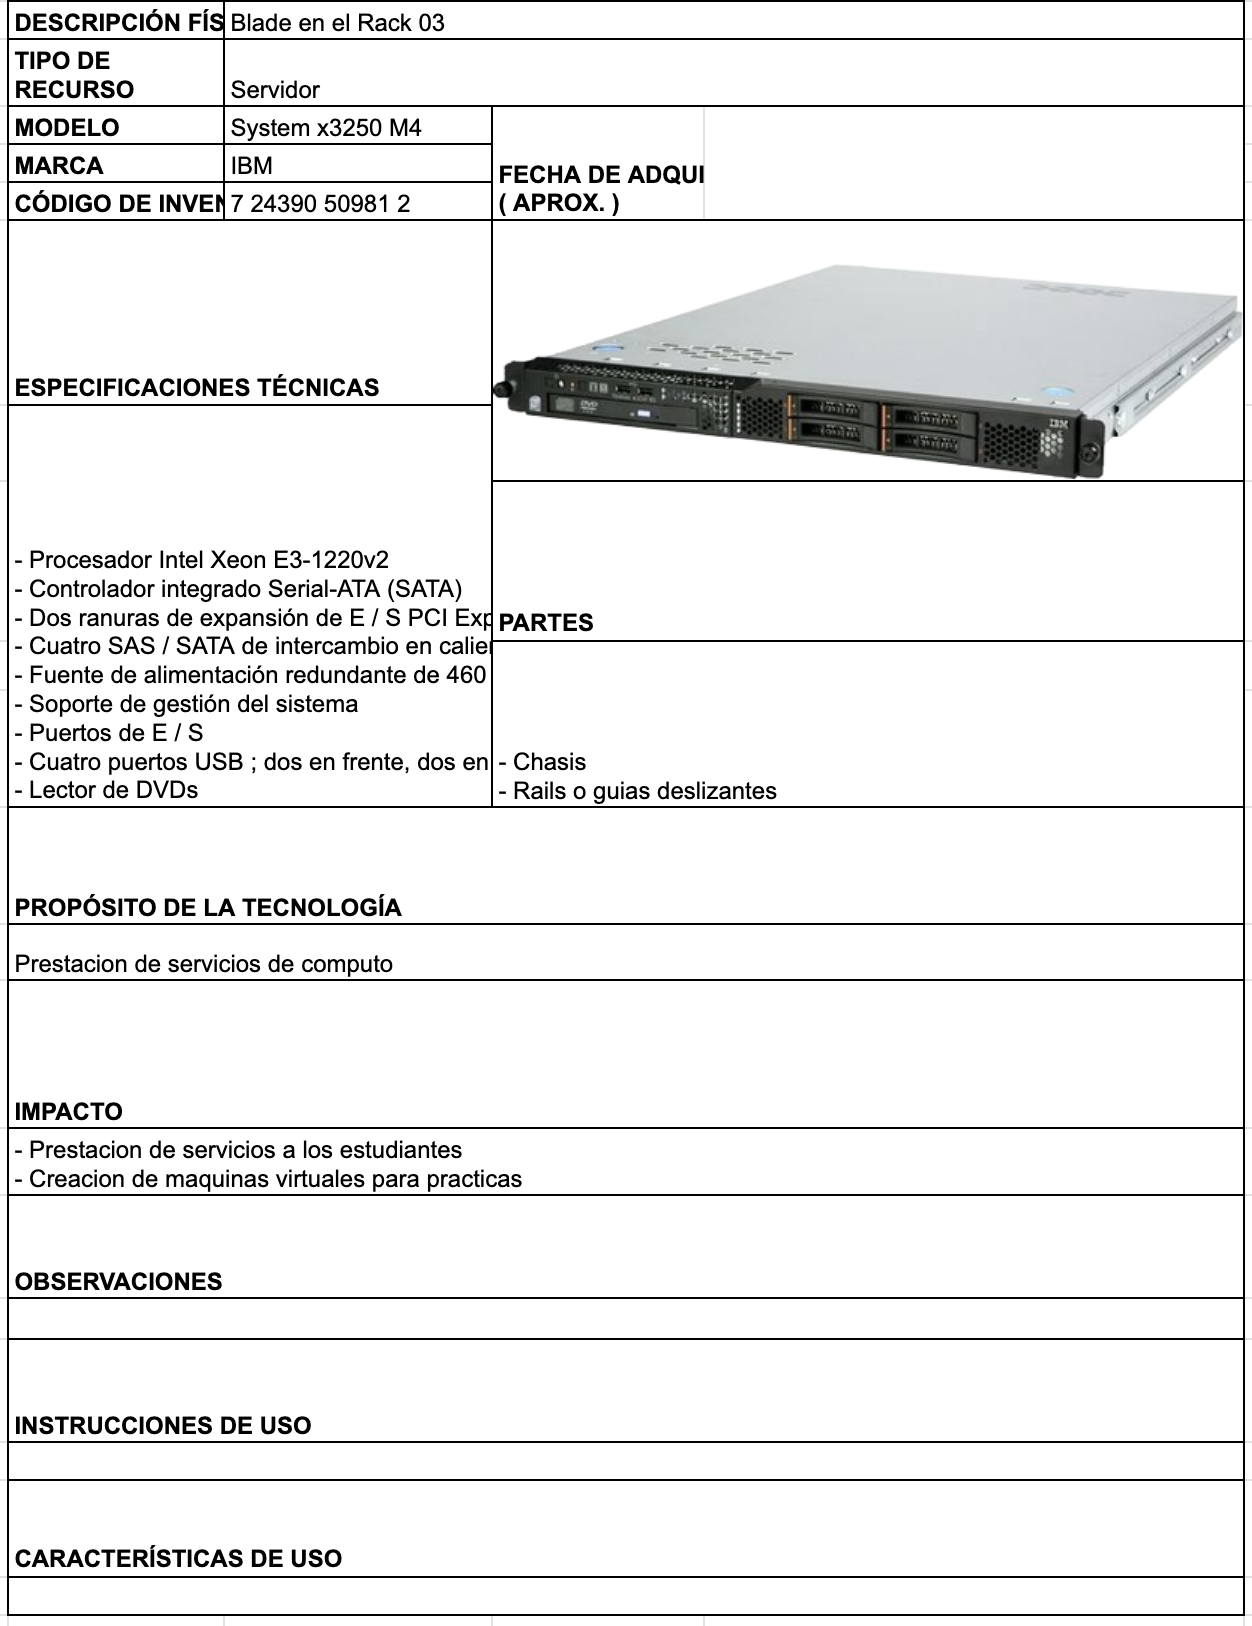
\includegraphics[width=0.25\textwidth,height=4cm,keepaspectratio]{tablas-images/cp1/racks/rack-1.png}} \\ \cline{1-1}
\textbf{MODELO:} System x3250 M4 & \\ \cline{1-1}
\textbf{MARCA:} IBM & \\ \cline{1-1}
\textbf{CÓDIGO DE INVENTARIO:} 7 24390 50980 & \\ \cline{1-1}
\textbf{NUMERO EN CPD:} 54 & \\ \hline
\multicolumn{2}{|l|}{\textbf{ESPECIFICACIONES TÉCNICAS}} \\ \hline
\multicolumn{2}{|p{0.95\textwidth}|}{
\footnotesize
- Procesador Intel Xeon E3-1220v2
- Controlador integrado Serial-ATA (SATA)
- Dos ranuras de expansión de E / S PCI Express
- Cuatro SAS / SATA de intercambio en caliente de 2,5 pulgadas
- Fuente de alimentación redundante de 460 vatios
- Soporte de gestión del sistema
- Puertos de E / S
- Cuatro puertos USB ; dos en frente, dos en la parte trasera
- Lector de DVDs
} \\ \hline
\multicolumn{2}{|l|}{\textbf{PROPÓSITO:} Prestacion de servicios de computo} \\ \hline
\multicolumn{2}{|p{0.9\textwidth}|}{\textbf{IMPACTO:} - Prestacion de servicios a los estudiantes
- Creacion de maquinas virtuales para practicas} \\ \hline
\multicolumn{2}{|p{0.9\textwidth}|}{\textbf{OBSERVACIONES:}  Ninguna} \\ \hline
\end{tabular}
\end{table}

% Rack 3
\begin{table}[H]
\centering
\caption{Ficha técnica --- Rack 3}
\label{tab:rack-3}
\begin{tabular}{|p{0.6\textwidth}|p{0.3\textwidth}|}
\hline
\multicolumn{2}{|l|}{\textbf{DESCRIPCIÓN FÍSICA:} Servidor tipo rack} \\ \hline
\textbf{TIPO DE RECURSO:} Servidor & 
\multirow{5}{*}{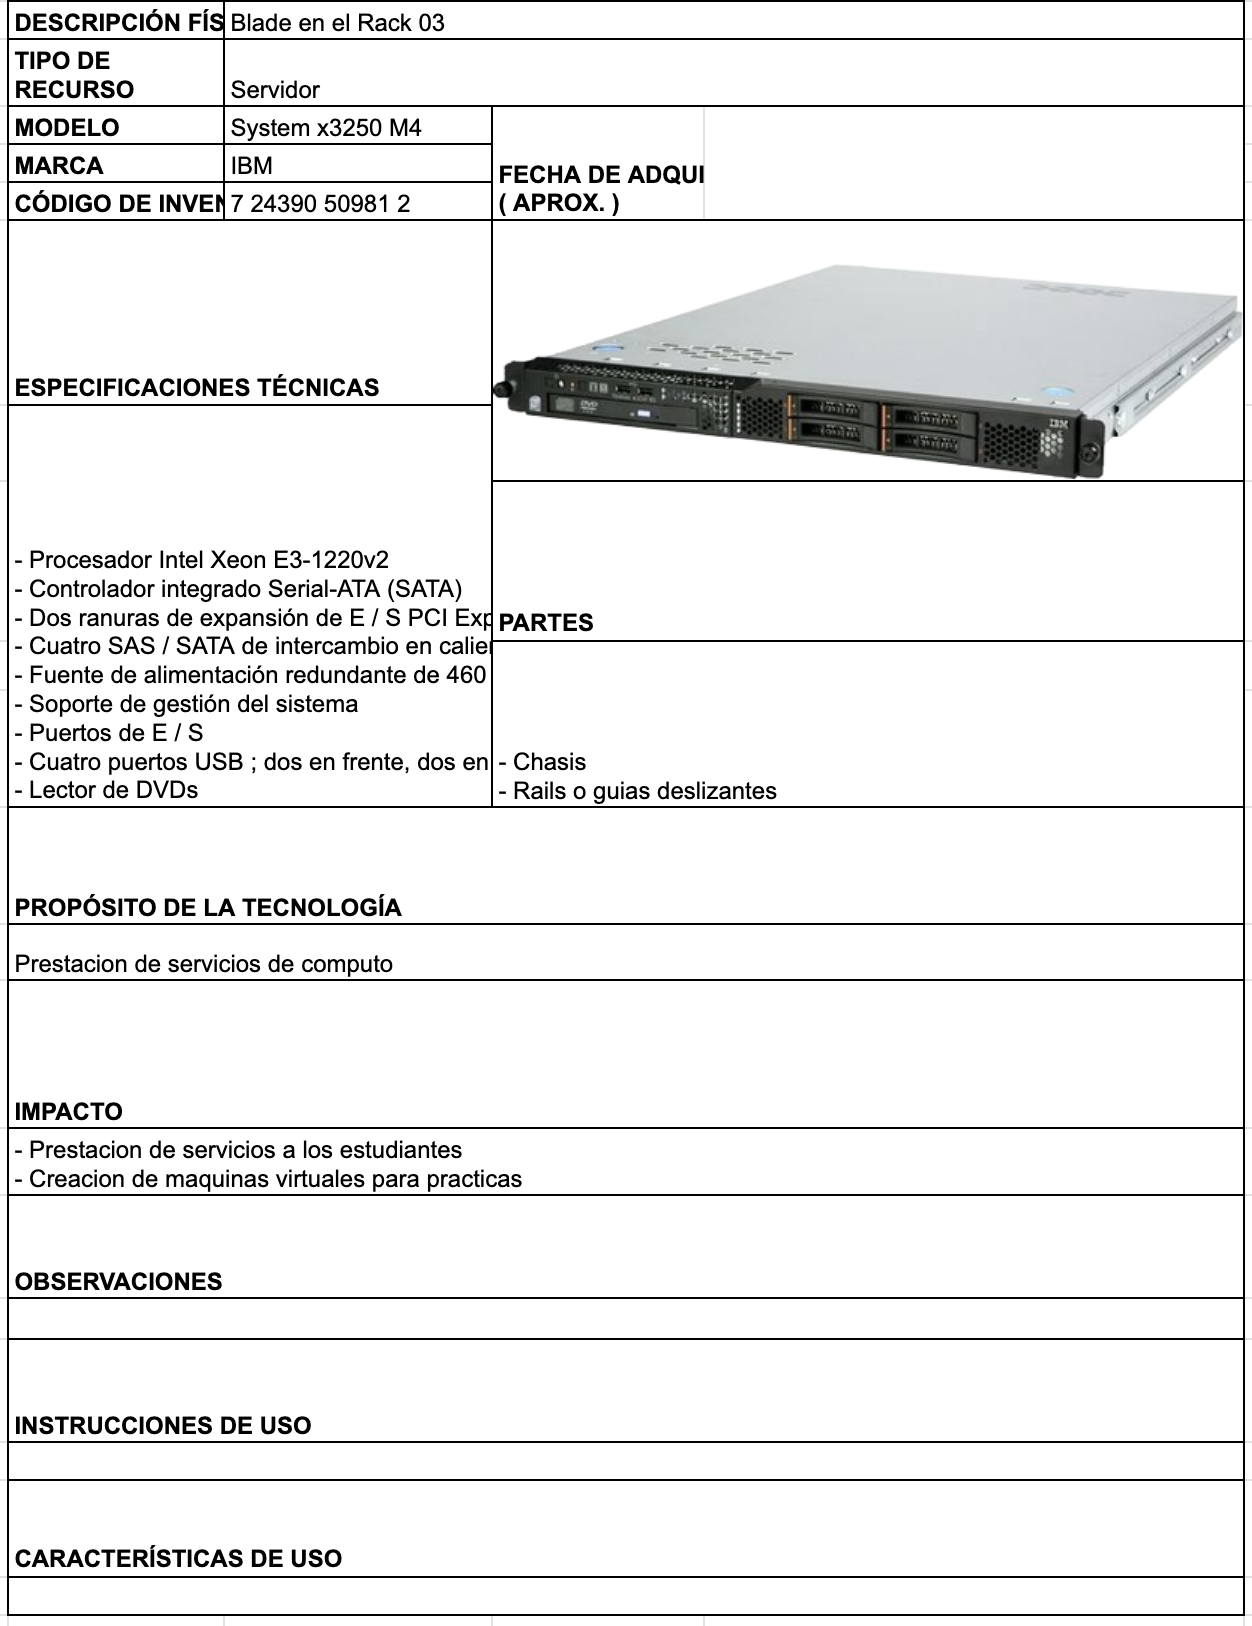
\includegraphics[width=0.25\textwidth,height=4cm,keepaspectratio]{tablas-images/cp1/racks/rack-1.png}} \\ \cline{1-1}
\textbf{MODELO:} System x3250 M4 & \\ \cline{1-1}
\textbf{MARCA:} IBM & \\ \cline{1-1}
\textbf{CÓDIGO DE INVENTARIO:} 7 24390 50980 & \\ \cline{1-1}
\textbf{NUMERO EN CPD:} 53 & \\ \hline
\multicolumn{2}{|l|}{\textbf{ESPECIFICACIONES TÉCNICAS}} \\ \hline
\multicolumn{2}{|p{0.95\textwidth}|}{
\footnotesize
- Procesador Intel Xeon E3-1220v2
- Controlador integrado Serial-ATA (SATA)
- Dos ranuras de expansión de E / S PCI Express
- Cuatro SAS / SATA de intercambio en caliente de 2,5 pulgadas
- Fuente de alimentación redundante de 460 vatios
- Soporte de gestión del sistema
- Puertos de E / S
- Cuatro puertos USB ; dos en frente, dos en la parte trasera
- Lector de DVDs
} \\ \hline
\multicolumn{2}{|l|}{\textbf{PROPÓSITO:} Prestacion de servicios de computo} \\ \hline
\multicolumn{2}{|p{0.9\textwidth}|}{\textbf{IMPACTO:} - Prestacion de servicios a los estudiantes
- Creacion de maquinas virtuales para practicas} \\ \hline
\multicolumn{2}{|p{0.9\textwidth}|}{\textbf{OBSERVACIONES:} Ninguna} \\ \hline
\end{tabular}
\end{table}

% Rack 4
\begin{table}[H]
\centering
\caption{Ficha técnica --- Rack 4}
\label{tab:rack-4}
\begin{tabular}{|p{0.6\textwidth}|p{0.3\textwidth}|}
\hline
\multicolumn{2}{|l|}{\textbf{DESCRIPCIÓN FÍSICA:} Servidor tipo rack} \\ \hline
\textbf{TIPO DE RECURSO:} Servidor & 
\multirow{5}{*}{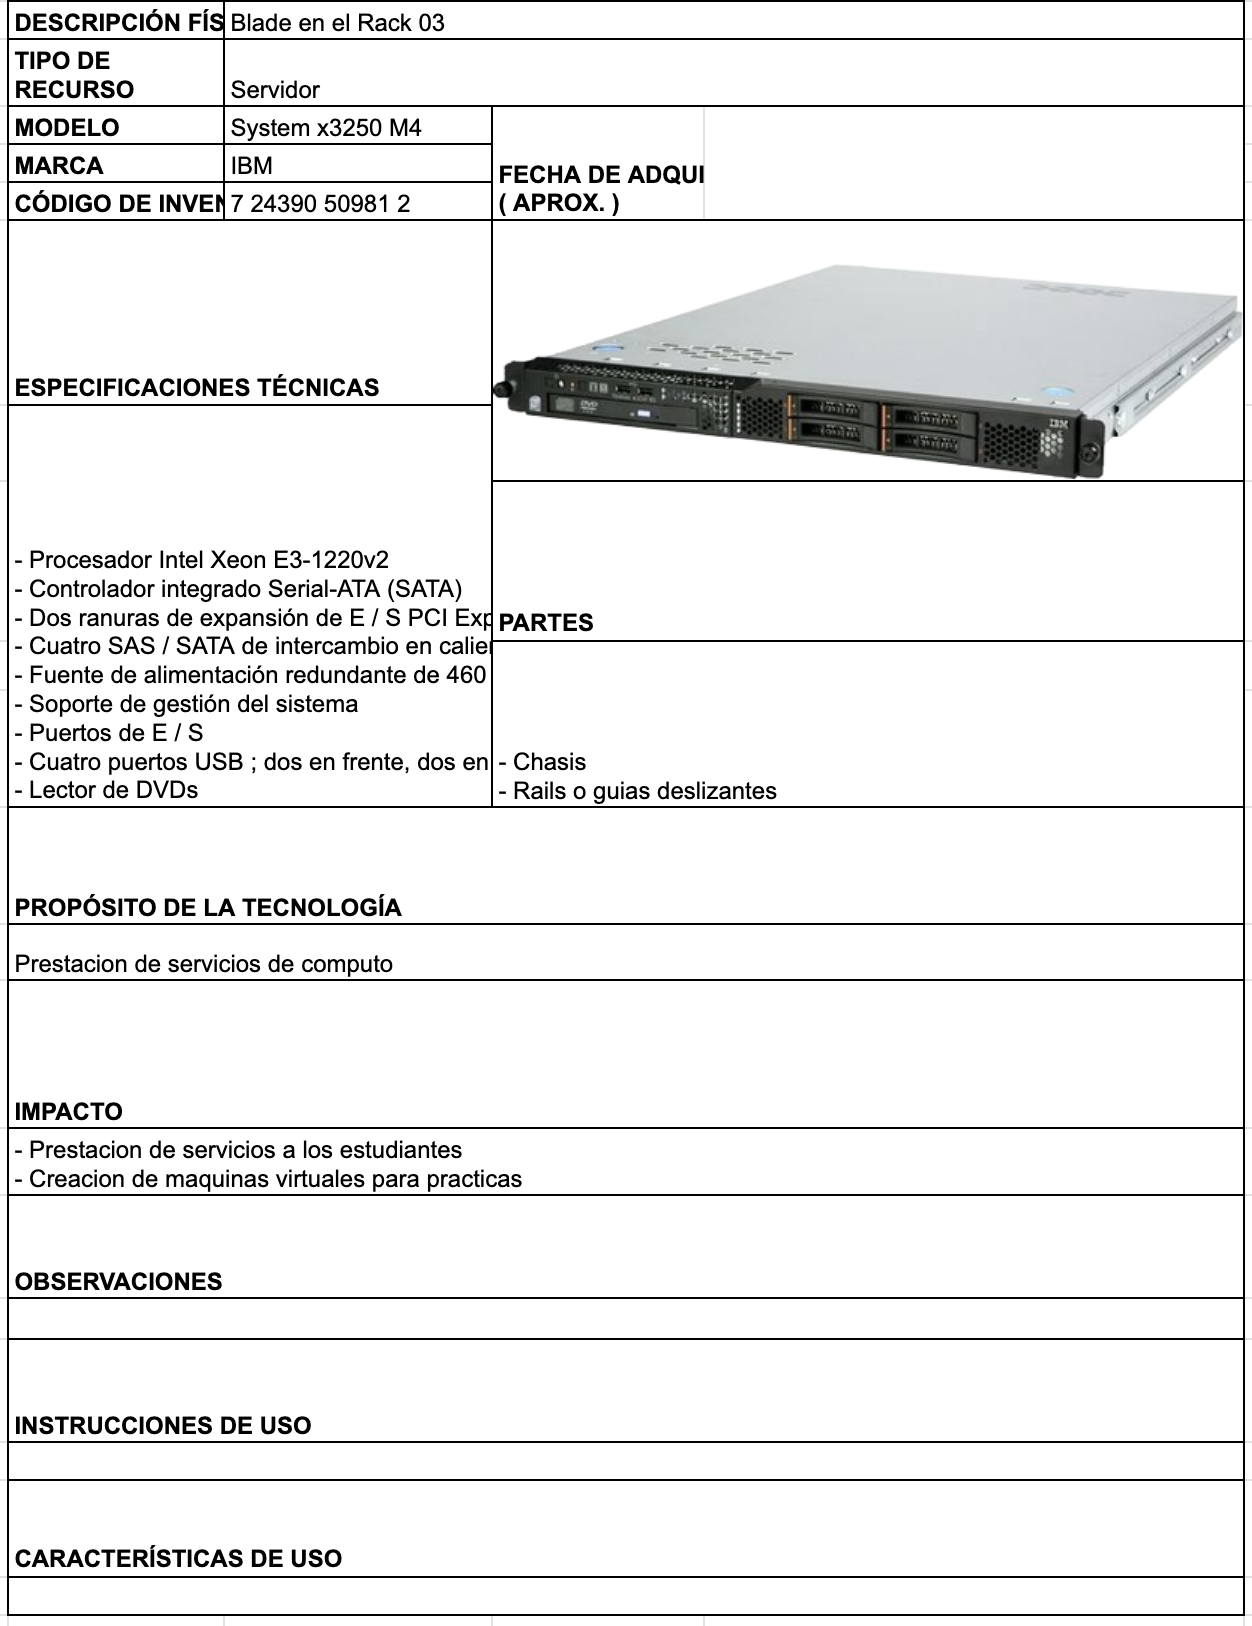
\includegraphics[width=0.25\textwidth,height=4cm,keepaspectratio]{tablas-images/cp1/racks/rack-1.png}} \\ \cline{1-1}
\textbf{MODELO:} System x3250 M4 & \\ \cline{1-1}
\textbf{MARCA:} IBM & \\ \cline{1-1}
\textbf{CÓDIGO DE INVENTARIO:} 7 24390 48735 & \\ \cline{1-1}
\textbf{NUMERO EN CPD:} 52 & \\ \hline
\multicolumn{2}{|l|}{\textbf{ESPECIFICACIONES TÉCNICAS}} \\ \hline
\multicolumn{2}{|p{0.95\textwidth}|}{
\footnotesize
- Procesador Intel Xeon E3-1220v2
- Controlador integrado Serial-ATA (SATA)
- Dos ranuras de expansión de E / S PCI Express
- Cuatro SAS / SATA de intercambio en caliente de 2,5 pulgadas
- Fuente de alimentación redundante de 460 vatios
- Soporte de gestión del sistema
- Puertos de E / S
- Cuatro puertos USB ; dos en frente, dos en la parte trasera
- Lector de DVDs
} \\ \hline
\multicolumn{2}{|l|}{\textbf{PROPÓSITO:} Prestacion de servicios de computo} \\ \hline
\multicolumn{2}{|p{0.9\textwidth}|}{\textbf{IMPACTO:} - Prestacion de servicios a los estudiantes
- Creacion de maquinas virtuales para practicas} \\ \hline
\multicolumn{2}{|p{0.9\textwidth}|}{\textbf{OBSERVACIONES:} Ninguna} \\ \hline
\end{tabular}
\end{table}


% Rack 5
\begin{table}[H]
\centering
\caption{Ficha técnica --- Rack 5}\label{tab:rack-5}
\begin{tabular}{|p{0.6\textwidth}|p{0.3\textwidth}|}
\hline
\multicolumn{2}{|l|}{\textbf{DESCRIPCIÓN FÍSICA:} Servidor tipo rack} \\ \hline
\textbf{TIPO DE RECURSO:} Servidor & 
\multirow{5}{*}{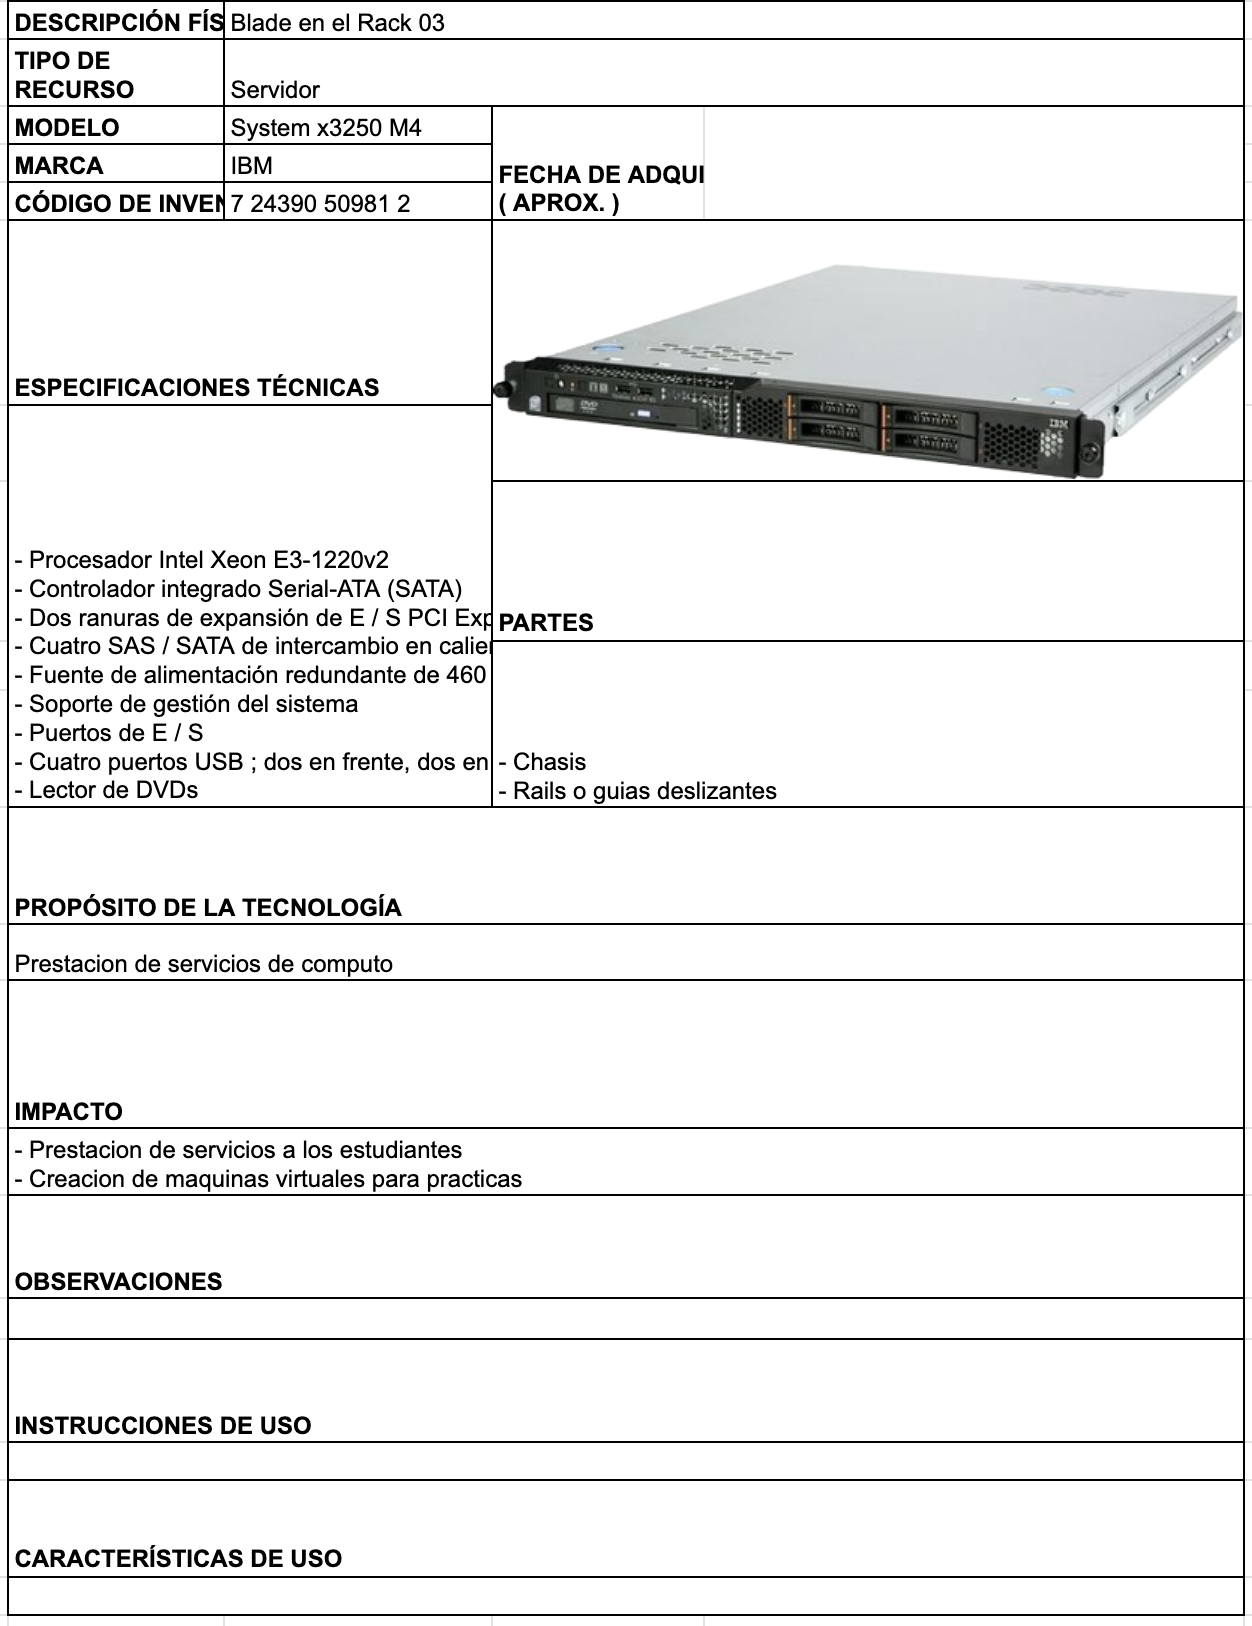
\includegraphics[width=0.25\textwidth,height=4cm,keepaspectratio]{tablas-images/cp1/racks/rack-1.png}} \\ \cline{1-1}
\textbf{MODELO:} System x3250 M4 & \\ \cline{1-1}
\textbf{MARCA:} IBM & \\ \cline{1-1}
\textbf{CÓDIGO DE INVENTARIO:} 51474 & \\ \cline{1-1}
\textbf{NUMERO EN CPD:} 52 & \\ \hline
\multicolumn{2}{|l|}{\textbf{ESPECIFICACIONES TÉCNICAS}} \\ \hline
\multicolumn{2}{|p{0.95\textwidth}|}{
\footnotesize
- Procesador Intel Xeon E3-1220v2
- Controlador integrado Serial-ATA (SATA)
- Dos ranuras de expansión de E / S PCI Express
- Cuatro SAS / SATA de intercambio en caliente de 2,5 pulgadas
- Fuente de alimentación redundante de 460 vatios
- Soporte de gestión del sistema
- Puertos de E / S
- Cuatro puertos USB ; dos en frente, dos en la parte trasera
- Lector de DVDs
} \\ \hline
\multicolumn{2}{|l|}{\textbf{PROPÓSITO:} Prestacion de servicios de computo} \\ \hline
\multicolumn{2}{|p{0.9\textwidth}|}{\textbf{IMPACTO:} - Prestacion de servicios a los estudiantes
- Creacion de maquinas virtuales para practicas} \\ \hline
\multicolumn{2}{|l|}{\textbf{OBSERVACIONES:} Ninguna} \\ \hline
\end{tabular}
\end{table}

% NAS 1
\begin{table}[H]
\centering
\caption{Ficha técnica --- NAS 1}\label{tab:nas-1}
\begin{tabular}{|p{0.6\textwidth}|p{0.3\textwidth}|}
\hline
\multicolumn{2}{|l|}{\textbf{DESCRIPCIÓN FÍSICA:} Sistema de almacenamiento conectado en red} \\ \hline
\textbf{TIPO DE RECURSO:} NAS (Network Attached Storage) & 
\multirow{5}{*}{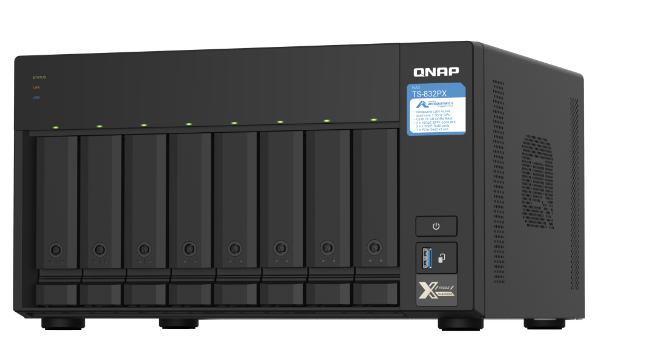
\includegraphics[width=0.25\textwidth,height=4cm,keepaspectratio]{tablas-images/cp1/NAS/nas-1.png}} \\ \cline{1-1}
\textbf{MODELO:} TS-832PX-4G & \\ \cline{1-1}
\textbf{MARCA:} QNAP & \\ \cline{1-1}
\textbf{CÓDIGO DE INVENTARIO:} Por definir & \\ \cline{1-1}
\textbf{FECHA DE ADQUISICIÓN (APROX.):} & \\ \hline
\multicolumn{2}{|l|}{\textbf{ESPECIFICACIONES TÉCNICAS}} \\ \hline
\multicolumn{2}{|p{0.95\textwidth}|}{
\footnotesize
- Procesador: Annapurna Labs Alpine AL-324, 4 núcleos, 1.7 GHz
- RAM: 4 GB DDR4 (expandible a 16 GB)
- Bahías: 8 bahías para discos duros SATA de 3.5" y 2.5"
- Ruido: Operación silenciosa con ventiladores de 120 mm
- Consumo: 50.8 W en funcionamiento, 27 W en reposo
- Puertos de Red: 2 x RJ45 2.5GbE, 2 x 10GbE
- Puertos USB: 1 x USB 3.2 Gen 1 frontal, 2 x USB 3.2 Gen 1 traseros
- Expansión: Ranuras PCIe para tarjetas de expansión adicionales
} \\ \hline
\multicolumn{2}{|p{0.9\textwidth}|}{\textbf{PROPÓSITO:} Proporcionar almacenamiento compartido y redundante a los usuarios y servidores dentro de una red} \\ \hline
\multicolumn{2}{|p{0.9\textwidth}|}{\textbf{IMPACTO:} - Proporciona almacenamiento y redundancia ( si la NAS falla, no hay disponibilidad de backups 
ni acceso a los archivos almacenados )} \\ \hline
\multicolumn{2}{|l|}{\textbf{OBSERVACIONES:} Ninguna} \\ \hline
\end{tabular}
\end{table}

% Firewall 1
\begin{table}[H]
\centering
\caption{Ficha técnica --- Firewall}\label{tab:firewall-1}
\begin{tabular}{|p{0.6\textwidth}|p{0.3\textwidth}|}\hline
\multicolumn{2}{|l|}{\textbf{DESCRIPCIÓN FÍSICA:} Sistema de seguridad de red} \\ \hline\textbf{TIPO DE RECURSO:} Firewall & 
\multirow{5}{*}{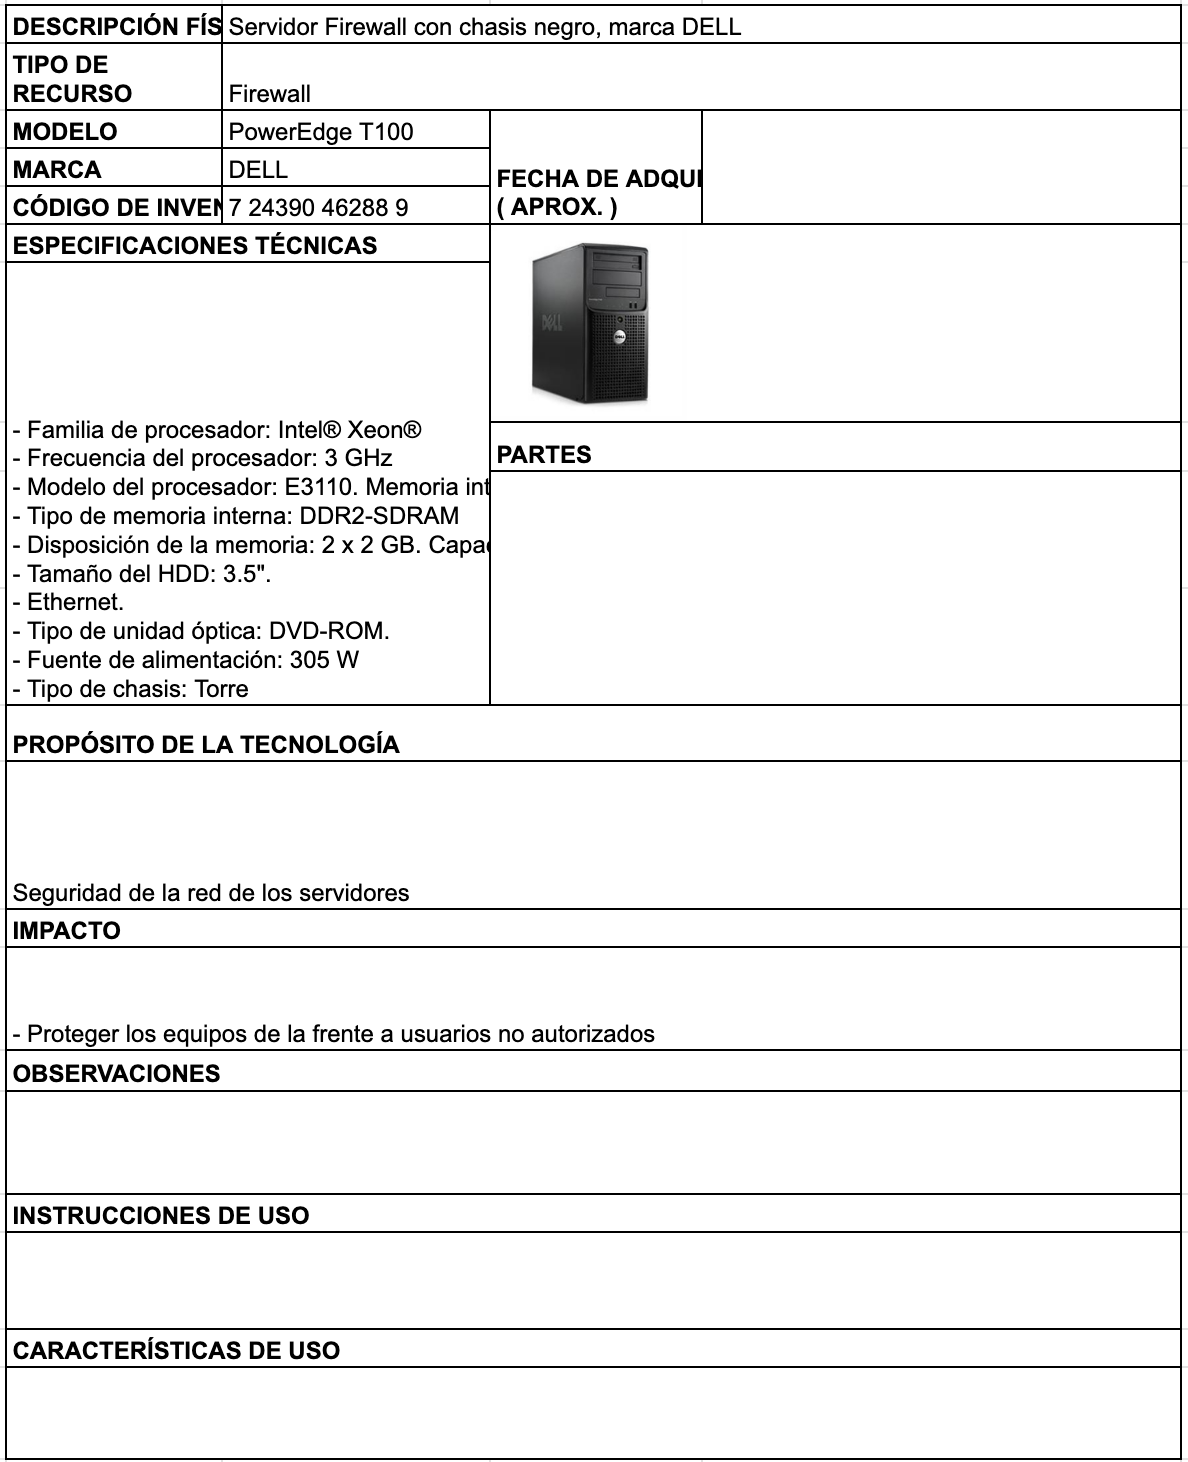
\includegraphics[width=0.25\textwidth,height=4cm,keepaspectratio]{tablas-images/cp1/firewall/firewall.png}} \\ \cline{1-1}
\textbf{MODELO:} PowerEdge T100 & \\ \cline{1-1}
\textbf{MARCA:} DELL & \\ \cline{1-1}
\textbf{CÓDIGO DE INVENTARIO:} 7 24390 46288 9 & \\ \cline{1-1}
\textbf{NÚMERO EN CPF:} No especificado & \\ \hline
\multicolumn{2}{|l|}{\textbf{ESPECIFICACIONES TÉCNICAS}} \\ \hline
\multicolumn{2}{|p{0.95\textwidth}|}{
\footnotesize
- Familia de procesador: Intel® Xeon®
- Frecuencia del procesador: 3 GHz
- Modelo del procesador: E3110. Memoria interna: 4 GB
- Tipo de memoria interna: DDR2-SDRAM
- Disposición de la memoria: 2 x 2 GB. Capacidad total de almacenaje: 1 TB
- Tamaño del HDD: 3.5". 
- Ethernet. 
- Tipo de unidad óptica: DVD-ROM. 
- Fuente de alimentación: 305 W 
- Tipo de chasis: Torre
} \\ \hline
\multicolumn{2}{|l|}{\textbf{PROPÓSITO:} Seguridad de la red de los servidores} \\ \hline
\multicolumn{2}{|l|}{\textbf{IMPACTO:} - Proteger los equipos de la frente a usuarios no autorizados} \\ \hline
\multicolumn{2}{|l|}{\textbf{OBSERVACIONES:} Ninguna} \\ \hline
\end{tabular}
\end{table}